\subsection{Seleção dos revestimentos}

Em praticamente todos os ramos de engenharia encontram-se problemas relacionados
ao desgaste. As perdas econômicas e consequentes de desgastes são generalizadas
e críticas. Estas não envolvem somente os custos de reposição, mas também os
custos de depreciação de equipamentos, perdas de produção, de competitividade e
de oportunidades de negócios.
O desgaste pode ser descrito como a perda progressiva de massa da superfície de
um corpo sólido causada pela ação mecânica, isto é, por contato e movimento
relativo de um contra-corpo sólido, líquido ou gasoso. De maneira mais
simplificada é a perda de material de uma ou de ambas as superfícies em contato
quando submetidas ao movimento relativo.

A avaliação da resistênica a erosão relativa entre materiais, um número de
fatores deve ser ser considerado. Além dos fatores óbvios como temperatura,
velicidade  e ângulo de impacto das partículas, tamanho e geometria dos grãos,
que podem ser controlados em testes normatizados pois a compreensão da
combinação das variabilidades  na performance é limitada.
O procedimento normatizado reduz o número de variáveis com a intenção de prever
uma base para comparação.
Modelos constituidos baseados em propriedades intrinsecas de cada sistema são
utilizados para prever a resistência à erosão e tiveram progresso ao longo dos
anos mas ainda estão em desenvolvimento. Modelos fluidodinâmicos utilizados para
prever o fluxo das partículas tem sido utilizados para aplicações típicas,
porém, os modelos necessitam ainda de valores medidos de taxas de erosão para
alimentação de banco de dados e para validação de resultados. O modelamento da
erosão tem um problema comum ao estudo dos diferentes tipos de desgaste, que tem
a ver com a grande quantidade de variáveis relacionadas com o tribo-sistema, que
podem influenciar a taxa de perda de material.

Quanto ao formato geométrico das partículas abrasivas, as de formas mais
irregulares encontradas na prática de engenharia produzem identaçoes mais
variáveis que as de formatos esféricos e muitas vezes as pontas se destacam e
se incorporam frequentemente  na superfície do alvo. Isto nos leva a uma camada
de compósito constituída do abrasivo com o metal de base cujo mecanismo de
erosão não é conhecido. A forma dessa camada de compósito entre partícula
incidente com o metal de base é de descoberta recente e o seu papel na erosão
dos metais ainda não é clara criando portanto uma outra variável antes não
prevista pelos modelos estudados.

O desgaste erosivo por impacto de partículas duras atua como fonte de
deterioração em componentes de equipamentos mecânicos industriais, sendo
prática comum a troca de peças que sofrem esses danos, e, portanto, fenômenos
que provocam desgastes, como corrosão, abrasão, erosão e cavitação, devem ser
considerados já nos projetos mecânicos e estruturais, não só na seleção dos
materiais a serem utilizados, mas também no aperfeiço\-amento do próprio
desenho.
A deterioração de componentes mecânicos se manifesta em função das
circunstâncias.

Os processos tribológicos que ocorrem no contato de duas superfícies que estão
em movimento relativo são muito complexos, uma vez que envolvem,
simultaneamente, o atrito e diferentes tipos e escalas de mecanismos de
desgaste e deformação. Apesar disso, na prática, atrito e desgaste são
fenômenos qualitativamente diferentes.

O atrito em sua definição mais elementar é a resistência ao movimento de um
corpo sobre o outro. É, também, a medida da dissipação de energia entre dois
corpos que deslizam e estão em contato. Ele geralmente é quantificado em termos
do coeficiente de atrito, que é uma medida adimensional obtida pela relação
entre força de atrito (força que se opõe ao movimento) e a carga ou peso do
corpo deslizante.

O atrito é causa de desgastes e de dissipação de energia em componentes
mecânicos, conduzindo à queda de desempenho e ao aumento do número de descartes
e reposiçoes, com os consequentes reflexos nos custos de operação e manutenção.
O controle do atrito e de seus efeitos conduz a uma considerável economia,
estimando-se que cerca de um terço dos recursos energéticos  mundiais sejam
usados, de alguma forma, para se superar o atrito.

Entre sólidos com movimento relativo entre si, a deterioração pode ocorrer de
duas maneiras: quando a diferença de dureza entre eles não é muito grande,
temos um desgaste, no material mais macio, provocado pelo atrito, com danos
superficiais e perdas de massa, em geral uniformes, o que provoca desajustes e
folgas indesejadas, como no caso dos mancais de deslizamento; quando os
materiais possuem durezas muito diferentes, temos a abrasão, um desgaste
superficial mais significativo, onde a perda de massa é mais rápida e em geral
irregular. Em componentes e instalaçoes em que temos superfícies sólidas, em
contato com fluidos em movimento relativo, temos outros tipos de deterioração.
A cavitação (do latim cavus,que significa um espaço vazio ou cavidade), é um
fenômeno observado tipicamente em equipamentos como turbinas e bombas
hidráulicas, e em válvulas e hélices de navios. Gases dissolvidos no líquido de
trabalho levam à formação e à implosão (colapso) de bolhas que provocam um
ataque às pás daqueles equipamentos, ataque este caracterizado pela perda
localizada de massa. No caso de fluidos em movimento, que contenham partículas
sólidas em suspensão, o contato com superfícies  internas leva a um desgaste
das mesmas conhecido como erosão. Tal desgaste, é provocado pelo choque das
partículas com as superfícies. Como conseqüência, temos uma redução da vida
útil e danos em tubulações e equipamentos. Quando o fenômeno da erosão age em
conjunto com o da corrosão, temos a chamada erosão-corrosão. Sabe-se que quando
da atuação do efeito sinérgico, a deterioração é maior que a soma dos outros
dois (efeito erosivo e efeito corrosivo) atuando individualmente. Em
componentes e estruturas expostos a meios agressivos, os materiais
constituintes estão sujeitos à corrosão. A corrosão é a causa mais importante
de deterioração de materiais,e decorre de reações químicas e eletroquímicas
agindo sobre eles e alterando, ao longo do tempo, seu aspecto, sua integridade
estrutural e sua massa. No que diz respeito a um estudo mais geral  da
deterioração de materiais, a área de pesquisa abrangente é chamada de
Tribologia e engloba os estudos que envolvem atrito, lubrificação e desgaste de
materiais. 

Tribologia é a ciência que faz a conexão entre todos os fatores associados aos
processos tribológicos e é voltada para o estudo do atrito, desgaste e
lubrificação de superfícies que estão em movimento relativo. É, portanto,
compreendida como a ciência e a tecnologia da interação de superfícies que
estão em movimento umas em relação às outras.

Alguns sistemas de classificação definem que os processos de desgaste podem ser
classificados em desgaste por deslizamento, rolamento, oscilação, impacto e
desgaste erosivo, dependendo da cinemática do sistema. Pode ser classificado
ainda em quatro mecanismos básicos: adesão, abrasão, fadiga superficial e reação
triboquímicaou ainda como de acordo com seu mecanismo em abrasão, adesão e
erosão.

A abrasão é normalmente provocada por partículas duras que estão incorporadas
em alguma superfície, ou por partículas que estão livres para deslizar e rolar
entre duas superfícies em contato deslizante. O desgaste abrasivo é causado
pela passagem destas partículas duras sobre a superfície e ocorre com perda
progressiva de material. O desgaste por abrasão pode ser definido como o
desgaste devido à penetração de partículas ou asperezas superficiais duras de
um contra corpo em uma superfície, durante o contato por deslizamento.

Partículas ou grãos abrasivos fazem parte das características inerentes de
muitos sistemas tribológicos. Dois grandes fatores que controlam a abrasividade
de uma partícula são tamanho e angularidade. Quanto maiores às dimensões das
partículas abrasivas maior será a taxa de desgaste da superfície atritada. Já a
angularidade ou afiabilidade descreve a forma das partículas, incluindo
saliências de sua superfície em termos do seu potencial de abrasão ou erosão.
Quanto mais agudo for o ângulo que constituem as arestas de um elemento
abrasivo, maior será a tendência de elevação na taxa de desgaste. A dureza,
tanto da partícula abrasiva como o da superfície de deslizamento, é outra
característica importante no processo de desgaste por abrasão. A taxa de
desgaste tende a diminuir com o aumento da dureza da superfície de
deslizamento. Nos metais, a presença de microconstituintes com elevada dureza
(alta concentração de carbono, carbetos, fases como a bainita e martensita)
contribuem para o aumento da resistência ao desgaste. Por outro lado, quanto
maior a dureza do agente abrasivo, tal como a de óxidos, por exemplo, maior
será o efeito de deterioração da superfície. 

A maneira como os grãos passam sobre a superfície determina a natureza do
desgaste abrasivo, que pode ser classificado como desgaste a dois ou a três.
Partículas incorporadas produzem abrasão a dois corpos (abrasão por
deslizamento) enquanto a ação de partículas abrasivas soltas é chamada de
abrasão a três corpos (abrasão por rolamento).

O desgaste abrasivo a dois corpos corresponde a um modelo de ferramenta de
corte, enquanto o desgaste abrasivo a três corpos envolve a ação de mecanismos
mais lentos de remoção de material. Neste caso, o material desgastado não é
removido por uma série de riscos como é o caso do desgaste abrasivo a dois
corpos. Em vez disso, a superfície gasta exibe uma topografia aleatória,
sugerindo a remoção gradual das camadas superficiais pelo contato sucessivo de
grãos. A taxa de remoção de material na abrasão a três corpos pode ser uma
ordem de magnitude menor do que a da abrasão a dois corpos porque as partículas
abrasivas soltas abradam a superfície apenas 10\% do tempo, enquanto passam 90\%
do tempo rolando. As partículas abrasivas podem interagir com a superfície de
desgaste através de diferentes mecanismos: microcorte, microfratura,
arrancamento de grãos, microssulcamento e formação de aresta.

Já o desgaste erosivo, a norma ASTM G76 define como a perda progressiva de
material de uma superfície sólida devido à interação mecânica entre superfícia
e um fluido, um fluido multicomponente, partículas líquidas ou sólidas
impactantes. A velocidade das partículas, o ângulo de impacto e o tamanho das
partículas abrasivas fornecem uma proporção de energia cinética da colisão das
partículas. Partículas de desgaste são formadas na erosão como resultado de
sucessivos impactos. Assim como no desgaste abrasivo, o desgaste por erosão
ocorre pela deformação plástica ou fratura frágil, dependendo do material a ser
erodido e das condições de operação. A relação entre taxa de desgaste e ângulo
de impacto é diferente para materiais dúcteis e frágeis. A forma das partículas
abrasivas também afeta a taxa de desgate. Partículas achatadas levam a uma
deformação mais localizada e por isso terão taxas de desgaste maiores do que
partículas arredondadas.

O impacto econômico da deterioração dos materiais metálicos, o desenvolvimento
de um sistema de revestimento e a viabialização da apliacação desse sistema
dentro dos equipamentos de uma unidade hidrelétrica, baixando os custos 
transporte e tempo de parada de máquina são os motivadores do estudo deste
projeto. Este trabalho foi desenvolvido com o fim de simularmos  experiências
práticas de laboratório, utilizando-se dos resultados e comparando-os com os da
literatura existente.

Como mencionado anteriormente os mecanismos de degsates são complexos além de
uma area de estudo vasta e particular de cada interação e equipamento. Diversas
são as formas de classificação e o que ocorre na prática é a sinergia dos
processos de deterioração e em muitos casos o processo de desgaste se inicia
por um mecanismo e se agrava por outro. Por este motivo vários testes forma
conduzidos de forma a selecionar o melhor sistema de revestimento para proteção
das superfícies das pás do tipo kaplan de turbinas hidrelétricos. Nesses testes
levou-se em consideração quatro diferentes formas de desgaste. Os procedimentos
foram conduzidos seguindo-se recomendações de normas internacionais a fim de se
obter resultados abrangentes.

Com o intuito de medir comparativamente o desempenho dos materiais selecionados
quanto a resistência à erosão foram conduzidos testes em um erodímetro com
granalha de óxido de alumínio seguindo as recomendações da norma ASTM G76.
Neste ensaio o abrasivo é dosado de forma precisa em um jato de ar comprimido
direcionado para a peça reproduzindo um desgaste por erosão de partícula
sólida.

O desgaste erosivo é um fenômeno complexo devido aos tempos de interação
partícula-superfície serem muito baixos, também chamado de período de
incubação, sendo, portanto um fenômeno de natureza fundamentalmente dinâmica.
Os parâmetros utilizados estão descritos na tabela \ref{tab:param_erosao}.


\begin{table}[H]
\centering
\begin{tabular}{|l|p{8cm}|}
 Parâmetros de ensaio e descrição das amostras  \\ \hline
 Granalha utilizada          &  Alumina eletrofundida angular  \\ \hline
 Diâmetro médio da partícula &  $375$ microns \\ \hline
 Velocidade da partícula     &  $50 m/s$ \\ \hline
 Temperatura de ensaio       &  $25^o C$ \\ \hline
 Tempo Total de ensaio       &  60 min \\ \hline
 Intervalo de medições       &  30 e 60 min \\ \hline
 Amostras 410-P              & Amostras em  aço inox AISI 410, dureza de 35 HRc,
 sem revestimento com acabamento polido, rugosidade $Ra<0,8$ \\ \hline
 Amostras 410-R              &  Amostras em aço inox AISI 410, dureza de
 35 HRc, sem revestimento com acabamento jateado, rugosidade $Ra>2,5$ \\ \hline
 Amostras WCCoCr-P           & Amostras com revestimento HVOF em Carboneto de
 Tungstênio com 10\% de Cobalto e 4\% de Cromo, dureza acima 1100 HV, acabamento
 polido e rugosidade $Ra<0,8$ \\ \hline
 Amostras WCCoCr-R           & Amostras com revestimento HVOF em Carboneto de
 Tungstênio com 10\% de Cobalto e 4\% de Cromo, dureza acima 1100 HV, acabamento
 como aspergido e rugosidade $Ra>2,5$ \\ \hline
 Amostras WCNi-P             & Amostras com revestimento HVOF em Carboneto de
 Tungstênio com 13\% de Niquel e 3\% de Cromo, dureza acima 1000 HV, resitência
 à cavitação, acabamento polido e rugosidade $Ra<0,8$ \\ \hline
 Amostra WCNi-R              &  Amostras com revestimento HVOF em Carboneto de
 Tungstênio com 13\% de Niquel e 3\% de Cromo, dureza acima 1000 HV, resitência
 à cavitação, acabamento como aspergido e rugosidade $Ra>2,5$ 
\end{tabular}
\caption{Parâmetros utilizados no ensaio de desgaste por erosão e descrição das
amostras}
\label{tab:param_erosao}

\end{table}

Os resultados foram medidos em perda de massa em 30 minutos de ensaio e em 60
minutos. Também foi controlado durente o processo o gasto de erodento que
também é embutido no cálculo do desgaste erosivo.

Para avaliação final utilizou-se somente os ensaios realizados nas amostras
Polidas atendendo a rugosidade  solicitada na norma pois o ensaio sofre muito
influência do acabamento. Dessa forma quanto mais fino o acabamento superficial
menor a influência no resultado do ensaio.

O resultado final é fornecido em perda de volume em mm³ – considerando as
densidades de cada material – e normalizado em relação ao gasto de erodente
durante o ensaio. A tabela \ref{tab:perda_vol} e o gráfico da figura
\ref{fig:ensaio_erosao} apresentam os resultados de desgaste erosivo compilados
para cada sistema.


\begin{table}[H]
\centering

\begin{tabular}{llll}
         & 410-P   & WCCoCr-P & WCNi-P  \\ \hline
 30 min  & 0,00965 & 0,00332  & 0,00544 \\ \hline
 60 min  & 0,01744 & 0,00486 &  0,00648  \\ \hline
 Total   & 0,02709 & 0,00818 &  0,01192   
\end{tabular}
\caption{Perda de volume em 30 e 60 minutos de ensaio para}
\label{tab:perda_vol}
\end{table}

\begin{figure}[h!]
\centering
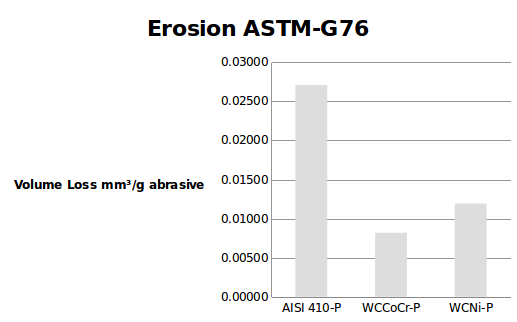
\includegraphics[width=0.8\textwidth]{method/figs/ensaio_erosao}
\caption{Ensaio de erosão: perda de volume acumulado por gasto de erodente.}
\label{fig:ensaio_erosao}
\end{figure}

Os ensaios de  desgaste abrasivo foram realizados emn um abrasômetro tipo roda
de borracha projetado e construído pela RIJEZA a fim de atender os requisitos
da norma ASTMN G65 que estabelece os procedimentos para a realização desse tipo
de ensaio. Foi utilizado o procedimento B da norma que recomentda uma rotação
de 200 rpm, carga de 130 N, tempo de 10 min e areia de sílica de granulometria
ASTM 100 como abrasivo. Cada corpo de prova é pesado antes e depois do ensaio
utilizando uma balança analítica de precisão 0,0001g. Com este ensaio é
possível obter a perda de volume de cada material o que interferirá no
desempenho relativo contra op desgaste de cada solução.

Para estes ensaios também se utilizou os mesmos materiais descritos para os
ensaios de erosão e cavitação. No entanto o ensaio foi realizado também para
qualificar a proposta de revestimento elastomérico sobre o coating HVOF. As
superfícies metalizadas foram preparadas com primer para receber a deposição do
revestimento Metaline 785, pulverizável, com dureza de 85 Shore A e resistente
à cavitação. Os sistemas utilizados nos testes destrutivos de abrasão estão
relacionados na tabela \ref{tab:ensaio_abrasao}. O resultados obtidos neste
ensaio estão apresentados no gráfico da figura \ref{fig:ensaio_abrasao}.

\begin{table}[H]
\centering
\begin{tabular}{|l|p{8cm}|}
Amostra     & Descrição \\ \hline
$WC_{10}Co_{4}Cr$   & Revestimento com composição química de 86\% Carboneto de
Tungstênio com 10\% de Cobalto e 4\% de Cromo \\ \hline
$WC_{13}Ni$         & Revestimento com composição química 88\%Carboneto de
Tungstênio com 13\% de Níquel e 3\% de Cromo \\ \hline
AISI 410            & Aço Inoxidável com composição química especificada na
norma AISI410 \\ \hline
Metaline 785        & Material base em aço Inoxidável, revestimento duplo de
$WC_{10}Co_{4}Cr$ e elastômero pulverizável Metaline 785 \\ \hline
\end{tabular}
\caption{Lista de Materiais utilizados no ensaio de abrasão conforme ASTM
G65-B.}
\label{tab:ensaio_abrasao}
\end{table}

\begin{figure}[h!]
\centering
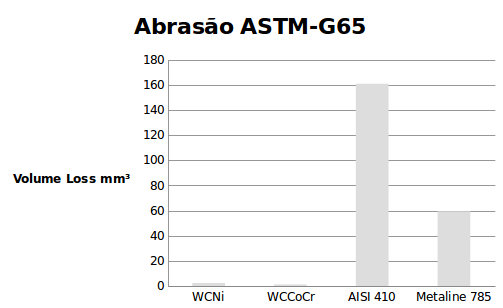
\includegraphics[width=0.8\textwidth]{method/figs/ensaio_abrasao}
\caption{Ensaio de abrasão: perda de volume para cada sistema testado.}
\label{fig:ensaio_abrasao}

\end{figure}


\subsection{Conclusão}
O conceito do projeto foi criado com a formulação das 4 perguntas que resumem a
finalidade do protótipo desenvolvido:

\begin{itemize}
  \item Quais as modificações necessárias aos equipamentos  de coating e
  jateamento para garantir acesso, funcionamento no circuito hidráulico e
  requisitos de segurança e meio ambiente?
  \item Quais as características do revestimento que podem ser influenciadas
  pelo ambiente proposto e devem ser constantemente controladas?
  \item Qual a classificação dos tipos de desgaste que estão danificando a
  superfícies das pás de UHE-Jirau e quais as regiões mais afetadas?
  \item Quais os sistemas de revestimentos mais adequados para combater o
  desgaste das pás, e quais modificações podem ser realizadas no Coating atual a
  fim de melhorar o desempenho do mesmo?
\end{itemize}

Os ensaios de abrasão mostraram a alta resistência à esse tipo de desgaste que a
superfície adquire após a aplicação do revestimento HVOF.  Tanto o revestimento
à base de WCNi como o revestimento à base de WCCoCr apresentaram taxas de
desgaste aproximadamente 70x e 120x menores que a superfície em aço INOX AISI
410 similar ao utilizado nas Pás da UHE Jirau. A resistência à erosão,
cavitação e corrosão dos dois revestimentos medidas em ensaio comparativo
mostraram que os coatings HVOF efetivamente aumentam substancialmente a
superfíce desgastada. Como dito anteriormente que o desgaste é um resultado da
somatória de cada mecanismo, também é importante considerar o acabamento da
superfíe que pode ser realizada a partir de produto elastpmérico pulverizável
Metalite – 785 que protege o revestimento quanto a caviação e mostra
resistência à abrasão intermediária entre os coatings HVOF e aço inoxidável.

O estudo do desgaste através de inspções mostraram que a severidade e a tipo é
diferente para diferentes regiões das pás. A proposta final é revestir as pás
nas regiões superiores, próximo à zona de entrada  do lado pressão com material
em WC-Ni com camada mínima de 0,2 mm e nas demais zonas das pás com material
WC-CoCr com camada mínima de 0,1 mm, utilizando um equipamento modelo DJ2700,
mais a aplicação de material elastomérico pulverizável para acréscimo da
proteção contra a cavitação e erosão da superfície. O equipamento de metalização
com combustão de GLP e Oxigênio ficará alocado como todos os seus insumos e
consoles no corredor de acesso à escotilha inferior da turbina. A superfíe será
preparada com jateamento abrasivo de Óxido de Alumínio, pré-aquecida se
necessário e o ambiente deverá ser monitorado e controlado através da montagem
de um sistema de exaustão e a utilização de instrumentos medidores de
temperatura e umidade relativa do ar.
